
%
% This document has designed to be read through as a PDF first.
% Click on the ``Typeset'' button in the toolbar to generate the PDF
% if it is not already visible.
%

%%% PREAMBLE %%%
% You probably want to skip to \begin{document} if this is your first time.

\documentclass[article,oneside]{memoir}
% This command goes at the beginning of every document
% [oneside,article] are two of many options that can be chosen
%   oneside makes each page have the same layout, for printing on only one side 
%     of the paper (change it to twoside to see the difference)
%   article means we're writing a short document only and won't be using special 
%     chapter headings
%   a4paper changes the page dimensions for A4 sized paper 

%%% PACKAGES %%%

\usepackage{graphicx} % Add graphics capabilities
\usepackage{booktabs} % ``Proper'' table layout
\usepackage{amsmath}  % Better maths support
\usepackage[colorlinks=false,linkcolor=red]{hyperref} % Hyperlink capabilities
%\usepackage{url}

\usepackage{memhfixc} % This package is required to resolve incompatibilities
                      % with the memoir class & the hyperref package
                      
\setlength{\oddsidemargin}{ 20pt}
\setlength{\textwidth}{440pt}
\setlength{\topmargin}{ 0pt}
\setlength{\headheight}{00pt}
\setlength{\headsep}{40pt}
\setlength{\textheight}{620pt}
%\usepackage{pdfsync}
% This package is used to tell TeXShop where things are in the PDF file.
% Command-click at any spot in the PDF and it will jump to the corresponding
% location in the source file.

\title {ENEE731 Project\\Normalized Cuts and Image Segmentation}
\author{Naotoshi Seo, sonots@umd.edu}
\date{November 8, 2006}


%%% BODY OF THE DOCUMENT: %%%
\begin{document}

\maketitle
% Generates a title based on the \title, \author, and \date commands in the preamble.

\chapter{Introduction}

Shi and Malik (1997) \cite{Shi} proposed the  Normalized Cuts for image segmentation problem, which is based on Graph Theory. 
This algorithm treats an image pixel as a node of graph, and considers segmentation as a graph partitioning problem. 
The Normalized Cuts algorithm measures both the total dissimilarity between the different groups as well as the total similarity within the groups. 
Amazingly, the optimal solution of splitting points is easily computed by solving a generalized eigenvalue problem. 

\chapter{Fundamental Idea}
A graph $\mathbf{G} = (\mathbf{V}, \mathbf{E}) $ can be partitioned into two disjoint sets, A, B. 
The degree of dissimilarity between these two pieces can be computed as 
\begin{equation}
cut(A, B) = \sum_{u \in A, v \in B} w(u, v). 
\end{equation}
where $w(u,v)$ is the similarity between node $u$ and $v$. 
The optimal bipartitioning of a graph is the one that minimizes this cut value. 
Finding the \textit{minimum cut} is a well-studied problem and there exist efficient algorithms for solving it. 
However, the minimum cut criteria favors cutting small sets of isolated nodes in the graph, and gives bad partition in some cases such as Fig. \ref{fig:cut}. 


\begin{figure}[htbp]
\begin{center}
    \includegraphics[height=3.5cm]{image/WS1.eps}
\caption{A case where minimum cut gives a bad partition.}
\label{fig:cut}
\end{center}
\end{figure}

Shi an Malik proposed a new measure o disassociation, the \textit{normalized cut} (Ncut): 
\begin{equation}
Ncut(A, B) =  \frac{cut(A, B)}{assoc(A, V)} + \frac{cut(A,B)}{assoc(B,V)}, 
\end{equation}
where $assoc(A,V) = \sum_{u \in A, t \in V} w(u, t) $ is the total connection from nodes in A to all nodes in the graph and $assoc(B,V)$ is similarly defined. 

Let $\mathbf{d}(i) = \sum_{j} {w(i,j})$  be the total connection from the node $i$  to all other nodes. Let $\mathbf{D}$  be an $N \times N$  diagonal matrix with $\mathbf{d}$  on its diagonal, $\mathbf{W}$  be an $N \times N$  symmetric matrix with $\mathbf{W}(i,j) = w(i,j)$. Then it turns out that we can minimize Ncut(A,B)  by
\begin{equation}
\min_{A,B} Ncut(A, B) = \min_\mathbf{y}
\frac{\mathbf{y}^T(\mathbf{D} - \mathbf{W})\mathbf{y}}{\mathbf{y}^T \mathbf{D} \mathbf{y}}. 
\end{equation}

If $\mathbf{y}$ is relaxed to take real values, the above equation can be minimized by solving the generalized eigen value system, 
\begin{equation}
 (\mathbf{D} - \mathbf{W})\mathbf{y} = \lambda \mathbf{D} \mathbf{y} . 
 \end{equation}
 Amazingly, the second smallest eigenvector $\mathbf{y}$ gives the solution of the normalized cut problem.

\chapter{Algorithm}

Given an image sequence $ \textbf{I} $. 
Construct a weighted graph $ \textbf{G} = (\textbf{V},\textbf{E}) $ 
whose each node is each pixel of the image $ \textbf{I} $.
Let $ N $ be the number of nodes (pixels), i.e., $ |\textbf{V}| $. 

\subsection{Step 1}
Construct an $ N \times N $ symmetric similarity matrix $ \textbf{W} $ as:

\begin{equation}
w_{ij} = exp{\frac{- ||\textbf{F}(i)-\textbf{F}(j)||^2_2}{\sigma_I^2}} *  
\left\{ \begin{array}{ll}
 exp{\frac{- ||\textbf{X}(i)-\textbf{X}(j)||^2_2}{\sigma_X^2}}  &\mbox{ if $ ||\textbf{X}(i)-\textbf{X}(j)||_2 < r $} \\
 0 &\mbox{ otherwise}
 \end{array} \right.
\end{equation}

\noindent
where $ \mathbf{X}(i) $ is the spatial location of node $ i $, i.e., the coordinates in the original image $ \textbf{I} $, and $ \textbf{F}(i) $ is a feature vector defined as:
\begin{itemize}
\item $ \textbf{F}(i) = 1 $ for segmenting point sets,
\item $ \textbf{F}(i) = \textbf{I}(i) $, the intensity value, for segmenting brightness (gray scale) images,
\item $ \textbf{F}(i) = [v,u \cdot s \cdot \sin(h), v \cdot s \cdot \cos(h)](i) $, where $ h,s,v $ are the HSV values, for color segmentation,
\item $ \textbf{F}(i) - [|\textbf{I} * f_1|,....,|\textbf{I} * f_n|](i) $, where the $ f_i $ are DOOG filters at various scales and orientations, for texture segmentation.
\end{itemize}

\noindent Let $ \mathbf{d}_{i} = \textstyle \sum_{j} w_{ij} $ be the total connection from node $ i $ to all other nodes. \\
Construct an $ N \times N $ diagonal matrix $ \textbf{D} $ with $ \mathbf{d} $ on its diagonal.

\subsection{Step 2}

Solve a generalized eigensystem, 
\begin{equation}
 (\mathbf{D} - \mathbf{W})\mathbf{y} = \lambda \mathbf{D} \mathbf{y} ,
 \end{equation}
 and get an eigenvector with the second smallest eigenvalue. 
 Fortunately, matlab has a function, eigs, to solve generalized eigensystems. 

\subsection{Step 3}

Use the eigenvector to bipartition the graph. In the ideal case, the eigenvector should only take on two discrete values, and the signs tell us exactly how to partition the graph ($ \mathbf{A} =\{ \mathbf{V}_i | \mathbf{y}_i > 0 \} $, $ \mathbf{B} = \{ \mathbf{V}_i | \mathbf{y}_i <= 0 \} $).

However, $ \mathbf{y} $ is relaxed to take real values, therefore, we need to choose a splitting point. There are several ways such as
\begin{itemize}
\item Take 0
\item Take median
\item Search a splitting point which results in that Ncut(A, B) is minimized. 
\end{itemize}
The splitting point which minimizes Ncut value also minimizes

\begin{equation} 
\frac{\mathbf{y}^T(\mathbf{D} - \mathbf{W})\mathbf{y}}{\mathbf{y}^T \mathbf{D} \mathbf{y}}
\end{equation}
where $ \mathbf{y} = (\mathbf{1} + \mathbf{x}) - b (\mathbf{1} - \mathbf{x}) $ where $ b = k / ( 1 - k ) $ where
$$
 \textstyle k = \frac{\sum_{x_i > 0} \mathbf{d}_i}{\sum_i \mathbf{d}_i}
$$
where $ \mathbf{x} $ is an N dimensional indicator vector, $ x_i = 1 $ if node $ i $ is in A and -1, otherwise.

To find the minimal Ncut, we need to try different values of splitting points. 
The optimal splitting point is generally around the mean value of the obtained eigenvector.
Fortunately, matlab has a function, fminsearch, which is suitable for this purpose. 

\subsection{Step 4}

Repeat bipartition recursively. Stop if \textit{Ncut} value is larger than a pre-specified threshold value (Large Ncut value means that there is no clear partition point any more). Furthermore, stop if the total number of nodes in the partition (\textit{Area}) is smaller than a pre-specified threshold value (this is another criteria added newly to the paper's algorithm.)


\newpage

\chapter{Experiments and Results}

\subsection{Gray scale Image}

Fig. \ref{fig:gray} shows the result of segmentation of a gray scale image. 
The image was obtained from \cite{dataset}. 

\noindent
\begin{center}
  \begin{figure}[ht]
  \begin{tabular}{@{} ccc @{}}

  \begin{minipage}{0.3\hsize}
   \begin{center}
    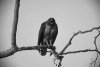
\includegraphics[]{image/s42049.eps}
    \\ (a)
   \end{center}
  \end{minipage}    &
   & 
   \\
  \begin{minipage}{0.3\hsize}
   \begin{center}
    \includegraphics[]{image/s42049-1.eps}
    \\ (b)
   \end{center}
  \end{minipage}    &
  \begin{minipage}{0.3\hsize}
   \begin{center}
    \includegraphics[]{image/s42049-2.eps}
    \\ (c)
   \end{center}
  \end{minipage}    &
  \begin{minipage}{0.3\hsize}
   \begin{center}
    \includegraphics[]{image/s42049-3.eps}
    \\ (d)
   \end{center}
  \end{minipage}    \\
  \begin{minipage}{0.3\hsize}
   \begin{center}
    \includegraphics[]{image/s42049-4.eps}
    \\ (e)
   \end{center}
  \end{minipage}    &
  \begin{minipage}{0.3\hsize}
   \begin{center}
    \includegraphics[]{image/s42049-5.eps}
    \\ (f)
   \end{center}
  \end{minipage}    &
  \begin{minipage}{0.3\hsize}
   \begin{center}
    \includegraphics[]{image/s42049-6.eps}
    \\ (g)
   \end{center}
  \end{minipage}    \\
 \end{tabular}
 \caption{(a) shows the gray scale original image of size 100x67. Image intensity is normalized to lie within 0 and 255. Subplots (b)-(g) show the components of the partition with $Ncut$ value less than 0.14, $Area$ size more than 220. Parameter setting: $ \sigma_I = 5.0, \sigma_X = 4.0, r =  1.5. $ }
 \label{fig:gray}
 \end{figure} 
\end{center}

\newpage

\subsection{Color Image}

Fig. \ref{fig:color} shows the result of segmentation of a color image. 
The image was obtained from \cite{dataset}. 

\noindent
\begin{center}
  \begin{figure}[ht]
  \begin{tabular}{@{} ccc @{}}

  \begin{minipage}{0.3\hsize}
   \begin{center}
    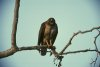
\includegraphics[]{image/sc42049.eps}
    \\ (a)
   \end{center}
  \end{minipage}    &
  \begin{minipage}{0.3\hsize}
   \begin{center}
    \includegraphics[]{image/sc42049-1.eps}
    \\ (b)
   \end{center}
  \end{minipage}    &
  \begin{minipage}{0.3\hsize}
   \begin{center}
    \includegraphics[]{image/sc42049-2.eps}
    \\ (c)
   \end{center}
  \end{minipage}    \\
  \begin{minipage}{0.3\hsize}
   \begin{center}
    \includegraphics[]{image/sc42049-3.eps}
    \\ (d)
   \end{center}
  \end{minipage}    &
  \begin{minipage}{0.3\hsize}
   \begin{center}
    \includegraphics[]{image/sc42049-4.eps}
    \\ (e)
   \end{center}
  \end{minipage}    &
  \begin{minipage}{0.3\hsize}
   \begin{center}
    \includegraphics[]{image/sc42049-5.eps}
    \\ (f)
   \end{center}
  \end{minipage}    \\
  \begin{minipage}{0.3\hsize}
   \begin{center}
    \includegraphics[]{image/sc42049-6.eps}
    \\ (g)
   \end{center}
  \end{minipage}    &
  \begin{minipage}{0.3\hsize}
   \begin{center}
    \includegraphics[]{image/sc42049-7.eps}
    \\ (h)
   \end{center}
  \end{minipage}    &
    \\
  \end{tabular}
 \caption{(a) shows the color original image of size 100x67. Each RGB intensity is normalized to lie within 0 and 255. Subplots (b)-(h) show the components of the partition with $Ncut$ value less than 0.21, $Area$ size more than 120. Parameter setting: $ \sigma_I = 5.0, \sigma_X = 6.0, r =  1.5. $ }
 \label{fig:color}
 \end{figure} 
\end{center}

\newpage

\subsection{Comparison}

Fig. \ref{fig:comparison} shows a comparison with a result of the program provided by Dr. Shi \cite{matlab}. The input image was also obtained from \cite{matlab}. 
The Dr. Shi's program took 77.6793 seconds for computation, but my program took 22.6640 seconds. 

\noindent
\begin{center}
  \begin{figure}[ht]
  \begin{tabular}{@{} ccc @{}}

  \begin{minipage}{0.3\hsize}
   \begin{center}
    
\includegraphics[width=3.5cm]{image/3.eps}
    \\ (a)
   \end{center}
  \end{minipage}    &
  \begin{minipage}{0.3\hsize}
   \begin{center}
    \includegraphics[height=4.2cm,width=4.8cm]{image/3-shi.eps}
    \\ (b)
   \end{center}
  \end{minipage}    &
                                  \\
  \begin{minipage}{0.3\hsize}
   \begin{center}
    \includegraphics[width=3.5cm]{image/3-1.eps}
    \\ (c)
   \end{center}
  \end{minipage}    &
  \begin{minipage}{0.3\hsize}
   \begin{center}
    \includegraphics[width=3.5cm]{image/3-2.eps}
    \\ (d)
   \end{center}
  \end{minipage}    &
  \begin{minipage}{0.3\hsize}
   \begin{center}
    \includegraphics[width=3.5cm]{image/3-3.eps}
    \\ (e)
   \end{center}
  \end{minipage}    \\
  \begin{minipage}{0.3\hsize}
   \begin{center}
    \includegraphics[width=3.5cm]{image/3-4.eps}
    \\ (f)
   \end{center}
  \end{minipage}    &
  \begin{minipage}{0.3\hsize}
   \begin{center}
    \includegraphics[width=3.5cm]{image/3-5.eps}
    \\ (g)
   \end{center}
  \end{minipage}    &
  \begin{minipage}{0.3\hsize}
   \begin{center}
    \includegraphics[width=3.5cm]{image/3-6.eps}
    \\ (h)
   \end{center}
  \end{minipage}   \\
  \end{tabular}
 \caption{(a) shows the color original image of size 160x160. (b) shows the result by Dr. Shi's program. Subplots (c)-(h) show the result by my program with $Ncut$ value less than 0.04, $Area$ size more than 1000. Parameter setting: $ \sigma_I = 5.0, \sigma_X = 6.0, r =  1.5. $ }
 \label{fig:comparison}
 \end{figure} 
\end{center}

\newpage

\chapter{Discussion}

My program worked reasonably fast for small images (e.g., 100 x 64), but it worked impractically for large images (e.g., 481 x 321). In particular, the calculation of eigen vectors and weight matrix required a lot of time, therefore, more efficient algorithm to compute them, and efficient tricks for memory management is required (they requires much of memory). Of course, we should consider implementing in low level languages such as C and using matlab mex, or running on powerful machines to shorten computation time, too.

My program worked faster than the program provided by Dr. Shi although his program is implemented by C and using matlab mex. It is probably because the Dr. Shi's program is more complicated or my matlab trick for fast computation worked well.

In order to obtain desired results, I had to carefully choose parameters. This is another optimization issue which must be solved in the future.

The electric version of this document and source codes is available at \url{http://note.sonots.com/SciSoftware/NcutImageSegmentation.html}

 \begin{thebibliography}{99}
 \bibitem{Shi} Jianbo Shi and Jitendra Malik, "Normalized Cuts and Image Segmentation," \textit{IEEE Transactions on PAMI}, Vol. 22, No. 8, Aug. 2000. 
 \url{http://www.cs.berkeley.edu/~malik/papers/SM-ncut.pdf}
\bibitem{Tutorial} Jianbo Shi, "Graph Based Image Segmentation Tutorial", \textit{CVPR}, June. 2004. 
  \url{http://www.cis.upenn.edu/~jshi/GraphTutorial/}
\bibitem{matlab} Jianbo Shi, "MATLAB Normalized Cuts Segmentation Code", 2006 (present). 
  \url{http://www.cis.upenn.edu/~jshi/software/}
\bibitem{dataset} D. Martin and C. Fowlkes and D. Tal and J. Malik, "A Database of Human Segmented Natural Images and its Application to Evaluating Segmentation Algorithms and Measuring Ecological Statistics", \textit{Proc. 8th Int'l Conf. Computer Vision}, vol. 2, pp. 416-423, July 2001. 
  \url{http://www.eecs.berkeley.edu/Research/Projects/CS/vision/bsds/}
\end{thebibliography}


\end{document}
